\section{Recognition Strategies}
\label{sec:background:recognition_strategies}

The \gls{icdar} robust reading competitions \citep{Lucas:2003iw, Lucas:2005bq, Shahab:2011hq} broke down the issue of text extraction into two sub-problems: text locating and character recognition. Most of the literature discussed in Section~\ref{sec:background:detection_strategies} focused within the text locating sub-problems; there were no expressions of interest in character recognition in \gls{icdar} 2003 and 2005 and only three in 2011 (the top system \citep{Liu:2005uw} scoring a correct recognition rate of 41.2\%). \todo{Refer to ICDAR 2013 and ICDAR 2015}.

It has been widely demonstrated that off-the-shelf commercial and open source OCR packages are able to correctly recognise text once the characters are extracted. Such usages include the use of the Tesseract \gls{ocr} \citep{Benami:2012jf} \todo{cite ICDAR2015}, TOCR and Readiris Pro \gls{ocr} \citep{XiangrongChen:2004ha}, ABBYY Fine Reader \gls{ocr} \citep{XiangrongChen:2004ha, Gatos:2005wd, Wang:2011tw, XiaomingHuang:2015fb}, TH-OCR \todo{cite from ICDAR2011}, INZI \todo{cite from ICDAR2011}, and TypeReader \gls{ocr} \citep{Li:2010dy} engines \todo{Link to relevant URLs for OCR engines}. Recent interest in developing novel general character recognition strategies has developed, such as the use of lexicon-free photo \gls{ocr} frameworks \citep{Lee:2016uy}.

\begin{figure}[h]
  \centering
  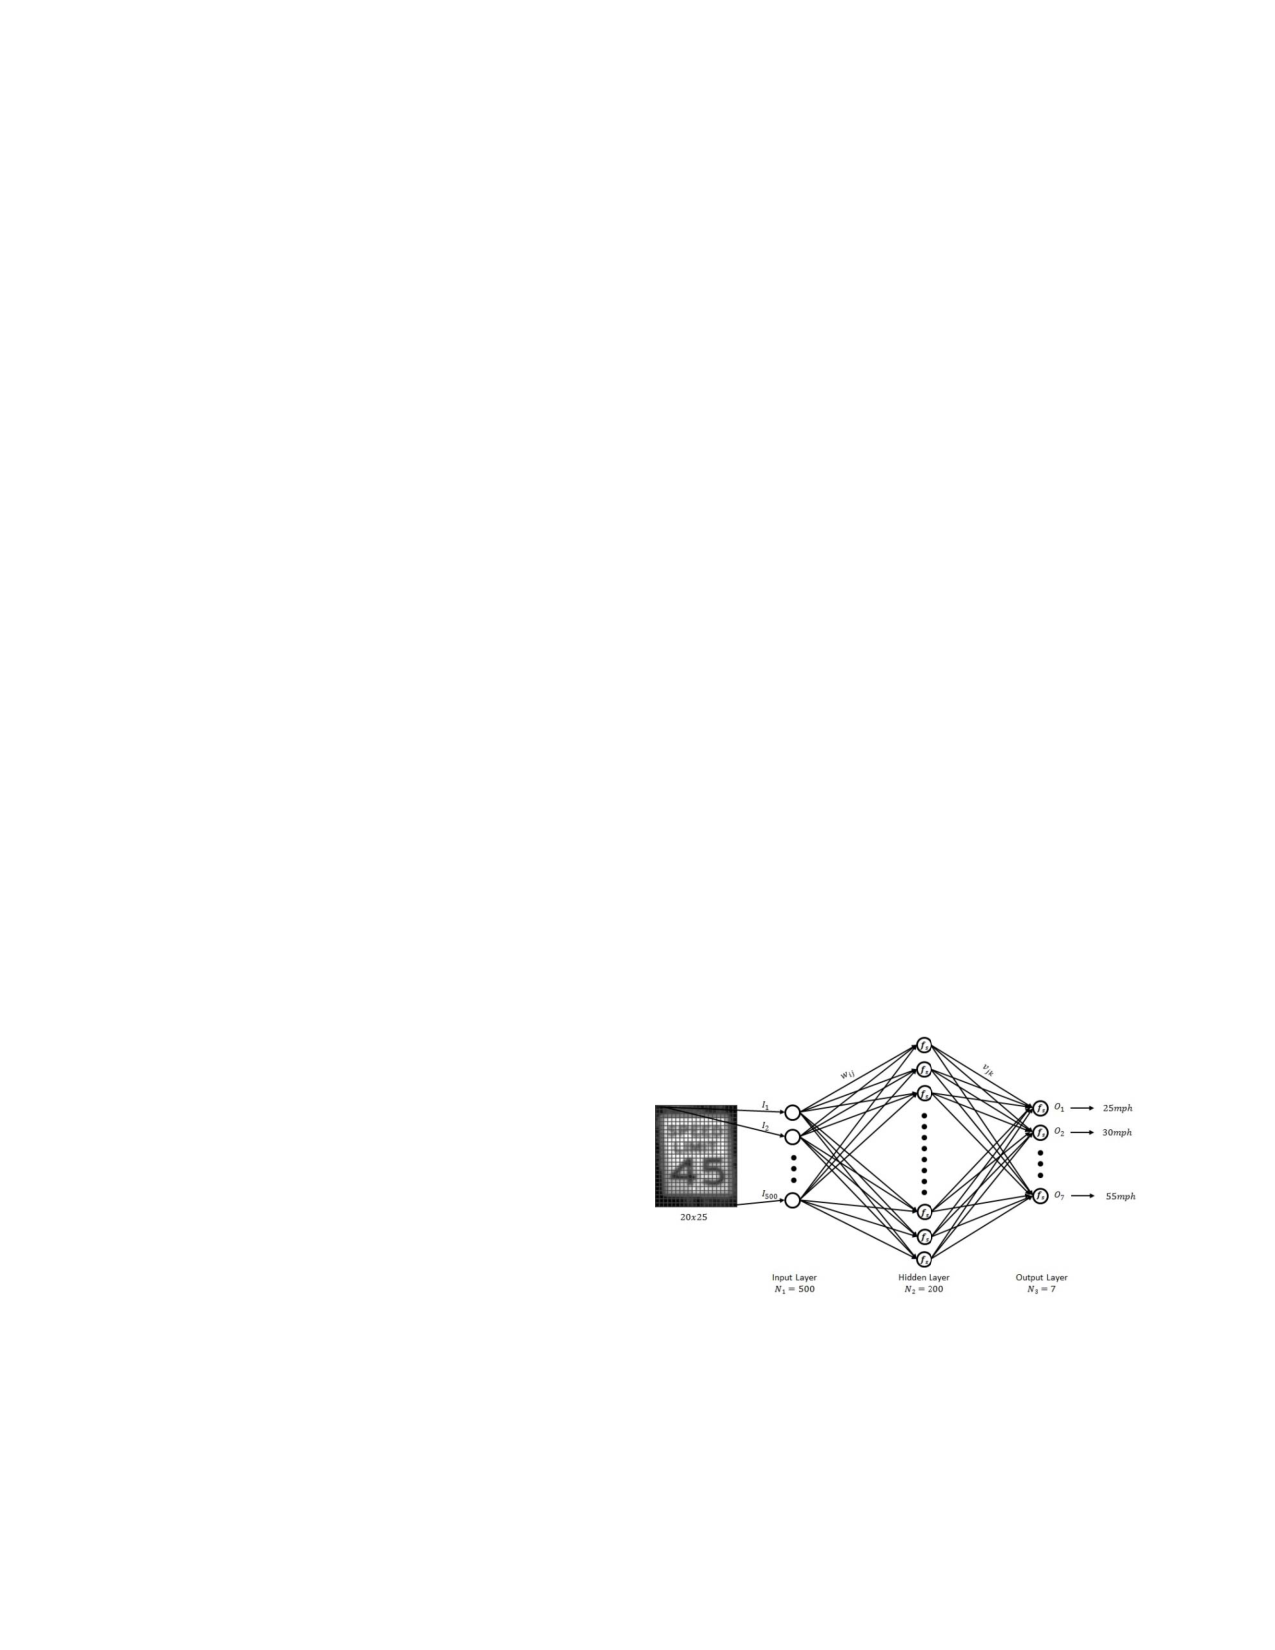
\includegraphics[width=0.75\textwidth]{images/background/kundu2015_nn}
  \caption[A NN designed to recognised speed limit signs]{The artificial \glsx{mlp} \gls{nn} designed in \citet{Kundu:2015vq} to recognise US-style speed limit signs.}
  \label{fig:background:recognition:kundu2015_nn}
\end{figure}

A \citeyear{Kundu:2015vq} study into \glsplx{tsr} to detect US-style speed limit signs achieved recognition without the use of any OCR packages. In \citep{Kundu:2015vq}, \citeauthor{Kundu:2015vq} were able to extract a speed limit sign via the use of \glspl{mser} and template matching. The resulting detected signs were scaled to a grayscaled size of $20 \times 25$ pixels and fed into a \glsx{mlp} \gls{nn} of 200 neurons in the hidden layer. The output layer of the network consisted of seven nodes, each representing the seven kinds of speed limit signs in US cities (25, 30, 35, 40, 45, 50, and 55 miles per hour). This architecture is shown in Figure~\ref{fig:background:recognition:kundu2015_nn}. When trained with 13,289 images of text cases and 4,319 non-text cases, the results showed that their recognition classier was able to correctly recognise speed limit signs with an accuracy of 98.04\%. Similar results were achieved using a feed-forward \gls{mlp} in \cite{Eichner:2008dw}, using UK/Poland style speed limits scaled to $20 \times 20$ pixels (grayscale) and 12 output layer neurons ($10 \dots 100$ kilometres per hour, the national speed limit sign, and non-sign neurons).

However, works in \gls{tsr} systems that utilise networks are generally non-generalisable, and only work in a limited context (i.e., by classifying speed limit signs of known outputs). In our context of \gls{rbn} recognition, we have a known character output range of 36 possibilities (0--9 and A--Z = 10 + 26). Beyond \gls{tsr} systems, however, we see the use of more generalisable networks: \citet{Netzer:2011to} trained neural network to recognise street number characters from Google Street View with higher precision and recall than that of \gls{hog} and the Tesseract \gls{ocr} engine, showing that the applicability of \glspl{nn} for recognition can outperform traditional means. \citet{Anagnostopoulos:2006wv} used a \gls{pnn} to recognise single characters of the same 36 possibility range (i.e., uppercase alphanumeric characters) corresponding to the input grayscale vector of $9 \times 12$ pixels ($9 \times 12 = 108$ input neurons) for a single character. Figure~\ref{fig:background:recognition:anagnostopoulos2006_nn} illustrates the \gls{pnn} architecture used in this study. Furthermore, investigations in comparing different architectures of \glspl{nn} for this context is given in \citet{Lee:2016uy}.

\begin{figure}[h]
  \centering
  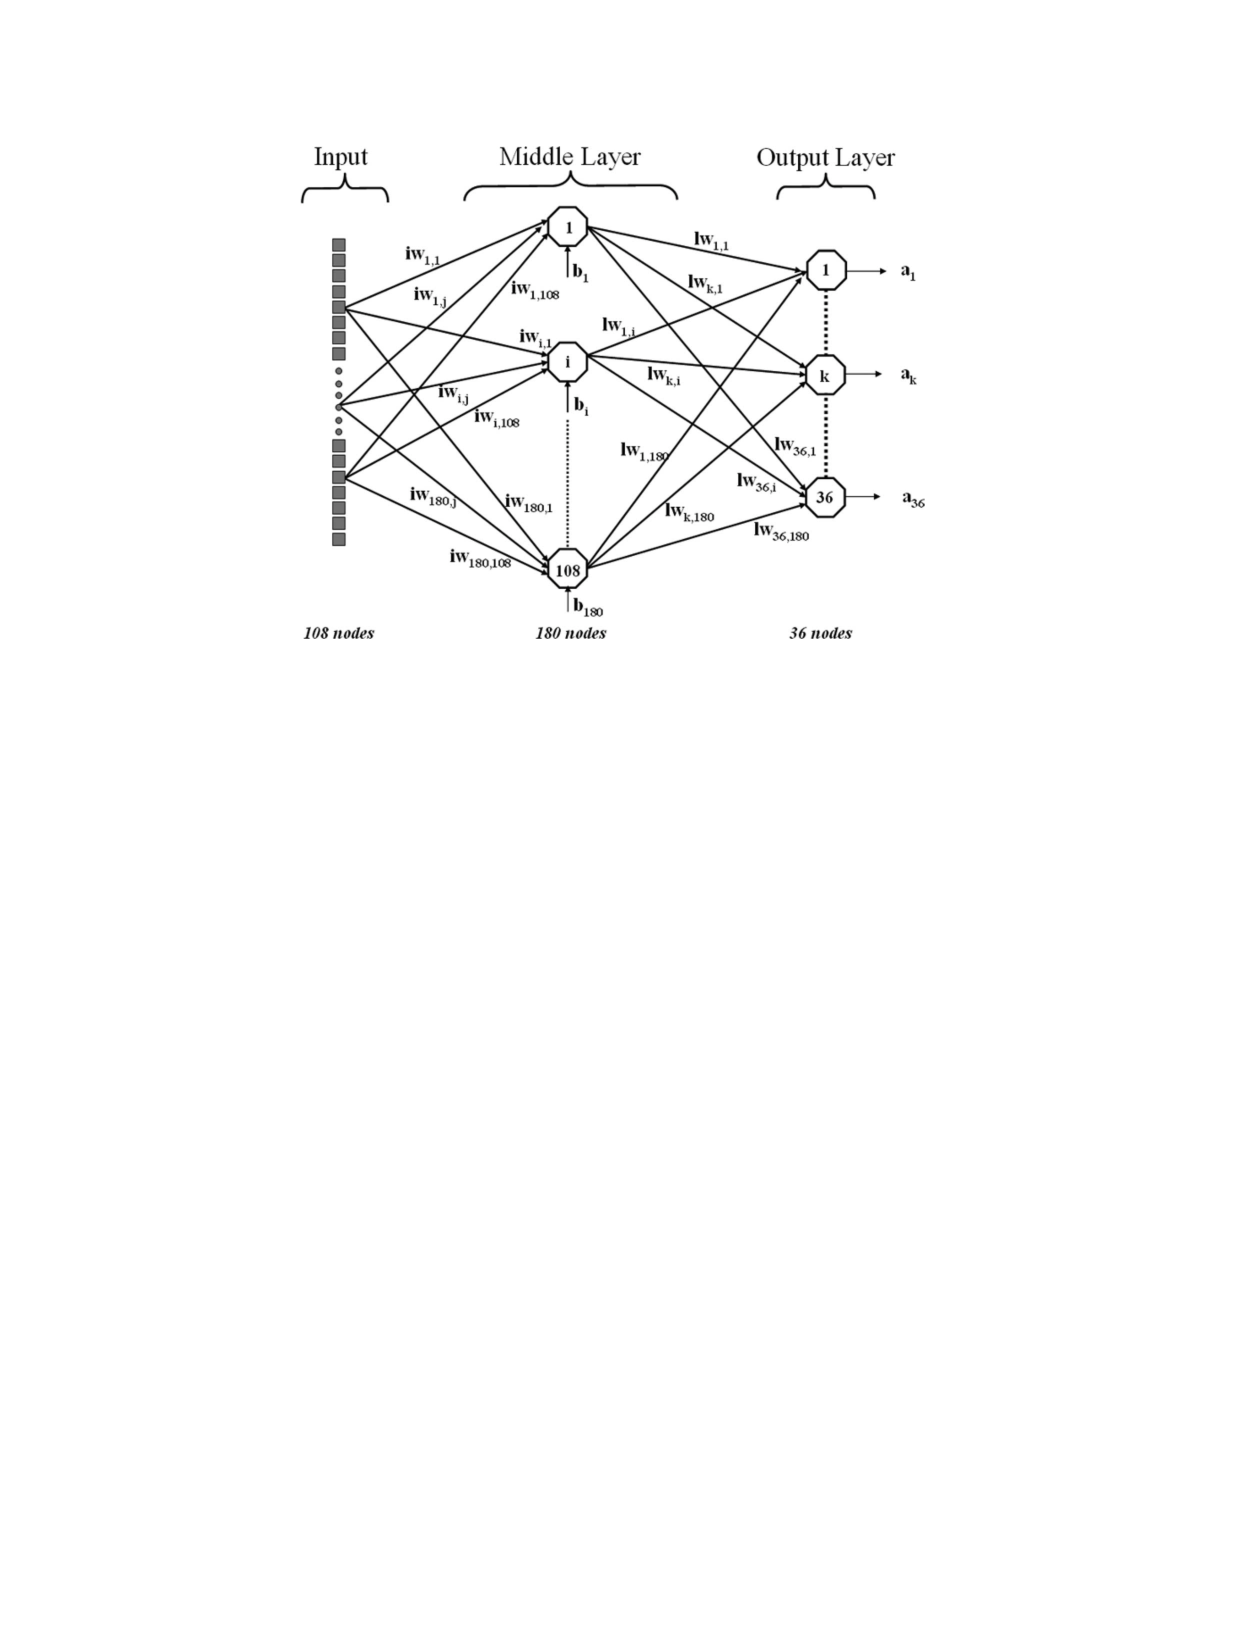
\includegraphics[width=0.75\textwidth]{images/background/anagnostopoulos2006_nn}
  \caption[A PNN used to recognise license plate characters]{\citet{Anagnostopoulos:2006wv} developed the architecture of a \gls{pnn} to determine a single character from within a license plate.}
  \label{fig:background:recognition:anagnostopoulos2006_nn}
\end{figure}

% Talk about BIB literature
% Talk about number plate literature
% Talk about speed sign NN literature